\documentclass[12pt]{article}

\usepackage{dftsl2}
\usepackage{amssymb}
\usepackage{amsmath}
\numberwithin{equation}{section}

\usepackage{graphicx,url}

%\usepackage[brazil]{babel}   
\usepackage[latin1]{inputenc}  

     
\sloppy

\title{Sistemas Lineares II}

\author{Igor Macedo Quintanilha\inst{1}, Roberto de Moura Estev�o Filho\inst{1}}


\address{Departamento de Eng. Elet. e de Comp. - Universidade Federal do Rio de Janeiro\\
  Rio de Janeiro - RJ - Brazil
  \email{\{igormq, robertomest\}@poli.ufrj.br}
}

\begin{document} 

\maketitle

\begin{resumo} 
Como relacionar a DFT de um conjunto de \textbf{N} amostras de um sinal com a Transformada de Fourier (\textit{FT}) do sinal?
\end{resumo}


\section{Nota��o}
Em todo o trabalho iremos considerar a seguinte nota��o:
\begin{itemize}
	\item Geral:
	\begin{itemize}
	\item $x(t)$ � o sinal cont�nuo
		\item $X(j\omega)$ � a \textbf{FT}
		\item $\omega(t) = 
			\begin{cases}
			    1,& -\frac{T_{0}}{2}\leq t \leq\frac{T_{0}}{2}\\0,& \mbox{caso contr�rio} 
		 	\end{cases}$
	\end{itemize}
	\item Janela de Observa��o:
	\begin{itemize}
		\item $W(j\omega)$ � a \textbf{FT} janela
		\item $y(t) = x(t)w(t)$ � a por��o de interesse
		\item $y(j\omega) = \mathcal{F}\{y(t)\}$
		\item $p(t) = \sum_{l=-\infty}^{\infty}\delta(t-lh)$ � o trem de impulsos
		\item $y^\star = y(t) \ast p(t)$ � o trem de impulsos modulados
		\item $y[n]$ s�o as amostras correspondentes
	\end{itemize}
\end{itemize}


\section{Multiplica��o pela janela} \label{sec:muljanela}
Para calcularmos o sinal $x(t)$ multiplicado pela janela $w(t)$, devemos encontrar a $\mathcal{F}\{w(t)\}$:
\begin{equation}
W(j\omega) = \int_{-\infty}^{\infty} w(t)\mathrm{e}^{-j\omega t}dt
\end{equation}
No entanto para $t > \left|\frac{T_{0}}{2}\right|$ o resultado � zero, ent�o:
\begin{subequations}
\begin{align}
W(j\omega) & = \int_{-\frac{T_{0}}{2}}^{\frac{T_{0}}{2}}\mathrm{e}^{-j\omega t}dt \nonumber \\ 
& = -\frac{1}{j\omega}\left(\mathrm{e}^{-j\omega T_{0}/_2}-\mathrm{e}^{j\omega T_{0}/_2}\right) = \frac{2\sin\left(\frac{\omega T_{0}}{2}\right)}{\omega} \nonumber \\
& = T_0 \frac{\sin\left(\frac{\omega T_0}{2}\right)}{\left(\frac{\omega T_0}{2}\right)} = T_0 sinc\left(\frac{\omega T_0}{2}\right)
\end{align}
\end{subequations}
Agora, multiplicando o sinal no tempo equivale a convolu��o na frequ�ncia:
\begin{displaymath}
y(t) = x(t) * w(t) \implies Y(j\omega) = X(j\omega) \star W(j\omega)
\end{displaymath}
Ent�o:
\begin{equation}
Y(j\omega) = \int_{\infty}^{-\infty}X(\tau)W(jw - \tau)d\tau
\end{equation}

\section{Amostragem}
Observamos que o sinal $p(t)$ � peri�dico, portanto podemos represent�-lo em sua s�rie de Fourier:
\begin{subequations}
\begin{align}
P_k &= \frac{1}{T_0}\int_{T_0}p(t)\mathrm{e}^{-jk\omega_0 t}dt \nonumber \\
& = \frac{1}{h}\int_{-h/_2}^{h/_2}\sum_{l=-\infty}^{\infty}\delta(t-lh)\mathrm{e}^{-jk\omega_0 t}dt,\quad\omega_0 = 2\pi/h \label{eqn:pk}
\end{align}
\end{subequations}
Como a integral est� definida dentro do per�odo fundamental, temos que a �nica solu��o n�o trivial � para $l=0$, portanto:
\begin{equation}
P_k = \frac{1}{h}\int_{-h/_2}^{h/_2}\delta(t)\mathrm{e}^{-jk\omega_0t}dt = \frac{1}{h}
\end{equation}
Com isso, temos o sinal $p(t)$ em sua s�rie de Fourier:
\begin{equation}
p(t) = \frac{1}{h}\sum_{k=-\infty}^{\infty}\mathrm{e}^{jk\omega_0t}
\end{equation}
Portanto, o sinal amostrado ser�:
\begin{equation}
y^\ast(t) = \frac{1}{h}\sum_{k=-\infty}^{\infty}y(t)\mathrm{e}^{jk\omega_0t} \label{eqn:amostrado}
\end{equation}
Aplicando a Transformada de Fourier no sinal \ref{eqn:amostrado}, temos:
\begin{displaymath}
Y^\ast(j\omega) = \frac{1}{h}\sum_{k=-\infty}^{\infty}\int_{-\infty}^{\infty}y(t)\mathrm{e}^{jk\omega_0t}\mathrm{e}^{-j\omega t}dt
\end{displaymath}
Utilizando a propriedade do deslocamento (?):
\begin{equation}
Y^\ast(j\omega) = \frac{1}{h}\sum_{k=-\infty}^{\infty}Y(j\omega-jk\omega_0)
\end{equation}
\section{Associando a $DTFT\{y[n]\}$ com a $\mathcal{F}\{y^*(t)\}$}
Realizando a DTFT do sinal $y[n]$:
\begin{equation}
Y(\mathrm{e}^{j\Omega}) = \sum_{n=-\infty}^{\infty}y[n]\mathrm{e}^{-j\Omega n}
\end{equation}
Utilizando uma outra abordagem para a transformada do sinal amostrado:
\begin{subequations}
\begin{align}
y^*(t) & = \sum_{l=-\infty}^{\infty}y(t)\delta(t-lh) \nonumber \\
& = \sum_{l=-\infty}^{\infty}y(lh)\delta(t-lh) \label{eqn:sinamos2}
\end{align}
\end{subequations}
Realizando a FT no sinal \ref{eqn:sinamos2}:
\begin{subequations}
\begin{align}
Y^\ast(j\omega) & = \sum_{l=-\infty}^{\infty}\int_{-\infty}^{\infty}y(lh)\delta(t-lh)\mathrm{e}^{-j\omega t}dt \nonumber \\
& = \sum_{l=-\infty}^{\infty}y(lh)\int_{-\infty}^{\infty}\delta(t-lh)\mathrm{e}^{-j\omega t}dt \nonumber \\
& = \sum_{l=-\infty}^{\infty} y(lh)\mathrm{e}^{-j\omega lh}
\end{align}
\end{subequations}
Para $\omega = \frac{\Omega}{h}$:
\begin{displaymath}
Y^\ast(j\omega) = \sum_{l=-\infty}^{\infty}y(lh)\mathrm{e}^{-j\Omega l} = Y(\mathrm{e}^{j\Omega})
\end{displaymath}
Adotando $y(lh) = y[l]$:
\begin{equation}
Y^\ast(j\omega) = \sum_{l=-\infty}^{\infty}y[l]\mathrm{e}^{-j\Omega l} = Y(\mathrm{e}^{j\Omega})
\end{equation}
\section{Relacionar a $DFT\{y[n]\}$ com $DTFT\{y[n]\}$}
\begin{subequations}
\begin{align}
DTFT: &\quad Y(\mathrm{e}^{j\Omega}) = \sum_{n=-\infty}^{\infty}y[n]\mathrm{e}^{-j\Omega n} \label{eqn:dtft}\\
DFT: &\quad Y[k] = \sum_{n=0}^{N-1}y[n]\mathrm{e}^{-j\left(\frac{2\pi}{N}\right)nk} \nonumber
\end{align}
\end{subequations}
Como $y[n] = 0$, para todo $(N-1) < n < 0$, temos em \ref{eqn:dtft}:
\begin{equation}
Y(\mathrm{e}^{j\Omega}) = \sum_{n=0}^{N-1}y[n]\mathrm{e}^{-j\Omega n}
\end{equation}
Para $\Omega = \frac{2\pi k }{N}$, finalmente temos:
\begin{equation}
Y(\mathrm{e}^{j\Omega}) = \sum_{n=0}^{N-1}y[n]\mathrm{e}^{-j\frac{2\pi k n}{N}} = Y[k]
\end{equation}

%\begin{figure}[ht]
%\centering
%
\includegraphics[width=.5\textwidth]{fig1.jpg}
%\caption{A typical figure}
%\label{fig:exampleFig1}
%\end{figure}

%\begin{table}[ht]
%\centering
%\caption{Variables to be considered on the evaluation of 5interaction
%  techniques}
%\label{tab:exTable1}
%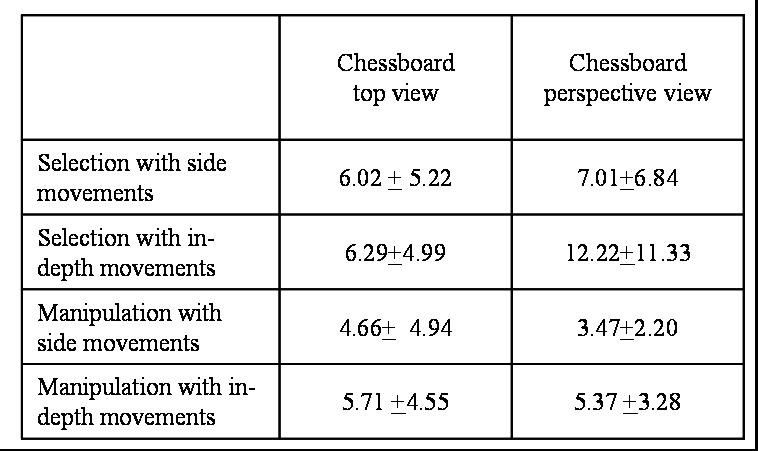
\includegraphics[width=.7\textwidth]{table.jpg}
%\end{table}

\section{Relacionar a $DFT\{y[n]\}$ com a $FT\{x(t)\}$}

All images and illustrations should be in black-and-white, or gray tones,
excepting for the papers that will be electronically available (on CD-ROMs,
internet, etc.). The image resolution on paper should be about 600 dpi for
black-and-white images, and 150-300 dpi for grayscale images.  Do not include
images with excessive resolution, as they may take hours to print, without any
visible difference in the result. 

\section{Relacionar a $DFT\{y[n]\}$ com a $DTFS\{x[n]\}$}
\begin{equation}
\frac{1}{N}DFT\{x[n]\} = DTFS\{x[n]\}|_{\Omega_0 = \frac{2\pi}{N}}
\end{equation}


\section{Refer�ncias}
\bibliographystyle{dftsl2}
\bibliography{dftsl2}

\end{document}
